%Language and Encoding
\usepackage[francais]{babel}
\usepackage[utf8]{inputenc}

%Images
\usepackage{graphicx} 

%Algorithm 
\usepackage{algorithmic}
\usepackage{algorithm}


%Info
\title{\textbf{Contrôle d'accès e le POSIX Access Control Lists(ACL)} \\ CS435 - Administration de Système }
\author{Dan Pham et Fabrício Nascimento}
\date{Octobre 2009}

\begin{document}

\maketitle
\newpage
%----------------------------------------------------------------------------
\section*{Introduction}
%Problème et solution plus simple
Quand on désire contrôler l'accès aux données dans un système de fichiers, il y a plusieurs moyens d’y parvenir. Par défaut, les systèmes POSIX (Portable Operation System Interface)\cite{ieee1,ieee2} ont un mécanisme qui permet d’associer chaque entité avec un ensemble de règles, lequel est composé par une séquence d'octet qui exprime les droits du propriétaire, de son groupe et des autres utilisateurs.

%Les limitations de cette solution
Ce mode, traditionnel, assez simple est capable de résoudre les problèmes les plus fréquents. Par contre, il pose des limitations aux administrateurs de systèmes qui pour exprimer leurs besoins doivent employer des configurations non évidentes. Certaines applications choisissent de développer leur propre système de droit comme le serveur FTP Proftp\cite{ftp} pour résoudre ce problèmes de droits.

% La solution ACL
Pour remédier à ces limitations, les systèmes UNIX peuvent employer les ACL. Cet article présente une exposition sur les ACL POSIX, ses modes de fonctionnement, ses qualités et désavantages. Le texte s’inspire de l'article d’Andreas Gruembacher\cite{aclsuse} qui a fait partit de l’équipe ayant ajouté le support aux ACL dans le noyaux Linux pour les systèmes de fichiers ext2 et ext3, qui sont les plus utilisés dans les monde UNIX.
\section{Le POSIX 1003.1}
 
Traditionnellement les systèmes qui implémentaient la norme POSIX avaient un système simple et puissant de permissions mais qui cependant posait certains problèmes. En effet, les différentes versions d'ACL disponibles étaient incompatibles entre elles.
 
Pour normaliser les problème de sécurité sur les systèmes POSIX (ACL en faisant partie), un groupe a été formé pendant la définition de la famille de normes POSIX 1003.1. Les premiers documents POSIX qui ont pris en compte ces questions étaient les documents 1003.1e (\emph{System Application Programming Interface}) et 1003.2c (\emph{Shell and Utilities}), cependant, le premier draft était trop ambitieux. En effet, le groupe responsable pour la normalisation avait divisé ses efforts sur un grand nombre de domaines qui comportaient les \emph{Access Control Lists} (ACL), les \emph{Audit}, les \emph{Capability},les \emph{ Mandatory Access Control }(MAC), et l'\emph{Information Labeling}\cite{aclsuse}.
 
En Janvier de 1998\cite{aclsuse} le financement pour ce projet à été suspendu, par contre, le travail n'était pas prêt. De toute façon le dixsèptieme draft a quand même été rendu public\cite{posix17}.
 
Après cette publication, des systèmes UNIX appelés "\emph{trusted}" (Trusted Solaris, Trusted Irix, Trusted AIX) ont été développés à partir du draft 17. Ces systèmes ne sont pas complètement compatibles entre eux. Heureusement aujourd'hui la plupart des systèmes UNIX et UNIX-like supportent les ACL. Ces implémentations sont usuellement compatibles avec le draft 17. Le projet TrustedBSD implémente aussi les ACL sur les système BSD. Les ACL sont apparues sur les Macs en 2003 avec la RELEASE MAC FreeBSD.
 
Les ACL sont une évolution du système de permissions traditionnel présent dans pratiquement tous les systèmes UNIX, alors, avant d'expliquer les ACL on va d'abord parler du modèle traditionnel.
 
\subsection*{Système de permissions traditionnel}
 
%Les groups et les permissions
Le modèle traditionnel POSIX offre trois classes d'utilisateurs qui sont: le propriétaire (\emph{owner}), le groupe propriétaire (\emph{group}) et les autres utilisateurs (\emph{others}). Chaque groupe a un octet que indique les permissions de lecture (\emph{\textbf{r}ead}), d'écriture (\emph{\textbf{w}rite}) et d'exécution (\emph{e\textbf{x}ecute}).
 
%Explication simple
Après les trois octets peut venir le \emph{Set User Id}, \emph{Set Group Id} et le \emph{Sticky Bit} qui peuvent être utilisés dans certain cas. Il faut faire attention avec le \emph{Sticky Bit}, il permet aux utilisateurs normaux d'exécuter les utilitaires comme l'administrateur(\emph{root}), donc une faille de sécurité dans une application utilisant le \emph{Sticky Bit} peut compromettre le système entier.
 
%Le droit du root
Seul le \emph{root} peut créer les groupes et changer les associations de groupes. Il peut aussi changer les propriétaires.
 
\subsection*{Les ACL}
 
%Definitions de base
Chaque ACL est une ensemble de règles d'accès. Dans une modèle de sécurité utilisant les ACL, si une entité fait une requête pour accéder aux données, il faut consulter les la liste d'ACL pour savoir si nous avons la permission pour l'opération demandé. Les règles possibles peuvent être consultées dans le tableau ci-dessous(\ref{entree}).

\begin{center}
\begin{tabular}{|l|l|}
  \hline
    \multicolumn{2}{|c|}{Les types de ACL} \\
  \hline
\textbf{Type d'entrée} & \textbf{format} \\
  \hline
Propriétaire & user::rwx \\
Utilisateur nommée & user:name:rwx \\
Groupe propriétaire & group::rwx \\
Groupe nommée & group:name:rwx \\
Masque & mask::rwx \\
Autres & other::rwx \\
  \hline
\end{tabular}
\label{tab:entree}
\end{center}
 
Les règles sont formées par un indicateur de classe (comme les classes du système traditionnel), l'identificateur pour préciser de quel utilisateur ou groupe on parle puis les octets de permissions.

Les ACL équivalentes au mode simple de permissions s'appellent les ACL minimales. Une ACL minimale possède 3 entrée (propriétaire, groupe propriétaire et autres) qui sont trivialement convertible. Si les ACL possèdent des entrées supplémentaires, ont les appelle ACL étendues. Toutes les ACL étendues doivent avoir une entrée masque et peuvent contenir théoriquement autant d'entrées que l'on désire. On verra après que ce numéro d'entrée peut-être limitée pour chaque implémentation et qu'il est aussi important pour les performances.

Quelquefois on a des application qui ne sont pas conscient de les ACL, ça veut dire qu'on doit crée une relation entre les ACL e le système traditionnelle de façon que ces application n'irons commencer a donner tout a coup et de façon inattendue plusieurs droits aux utilisateurs ou groupes. 

Quand on parle des ACL minimales ça n'arrive jamais, alors que la relation entre ces ACL e le système traditionnelle é directe. Par contre, dans les ACL étendu ça pose une problème. Pour le solutionner, on va changer le sens da classe groupe. Les propriétaire et les autres seront directement associe avec les classes de même nom, par contre, les entré de groupe et utilisateur nommé avec le groupe propriétaire seront tous associe avec la classe du groupe propriétaire. Par conséquent le sens du classe groupe propriétaire doit être redéfini comme le limite supérieur de les permission de chaque entrée dans les entrée associe a classe du groupe.

Comme dans les ACL étendues on peut avoir des entrées avec plusieurs utilisateurs et/ou groupes nomme, quelques de cette entrées peut-être contenir permissions qui la classe groupe n'aura pas, alors, on peut avoir une inconsistance dans certain cas. 

%@@

Ce question serais résoudre avec l'utilisation de une masque. Comme on peut l'observer dans le figure (\ref{fig:img_acl-mapping}), il y a deux cas:  Les ACL minimales où la classe groupe est référencée pour l'entrée du groupe propriétaire. Les ACL étendues de la classe groupe seront trouvées en faisant un masque avec les permissions du groupe propriétaire et les permissions des utilisateurs et groupe nommés. Cela rend difficile le calcul de classe groupe. 

\begin{figure}[htbp]
\centering
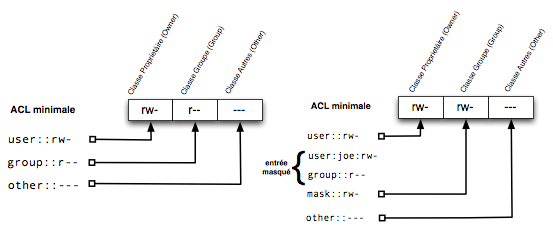
\includegraphics[height=3in]{img/acl-mapping.jpg}
\caption{caption}
\label{fig:img_acl-mapping}
\end{figure}
 
 
Pour assurer le cohérence, quand une application change les permissions (par exemple le commande \emph{chmod}) les ACL sont modifiée de façon a reproduire cette modification.
 
On a dit que la permission de la classe groupe est calculée comme la limite supérieure de tous les entrées dans le classe groupe. Avec les ACLs minimaux cette computation est simple, par contre, avec les ACLs étendu, on a besoin de masquer les permissions. Comme l'exemple de le tableau (\ref{tab:masquee}), les entrées de permission qui sont partie de la classe de groupe et qui aussi sont présente dans l'entrée masque sont applique effectivement. Si une permission était absent dans le masque, c'est a dire que aucun entrée de groupe (qui non le groupe du propriétaire) peut avoir ce permission, on dit dans ce cas qui la entrée est masquée.
 
\begin{center}
\begin{tabular}{|l|l|l|}
  \hline
    \multicolumn{3}{|c|}{La masque de permissionL} \\
  \hline
\textbf{Type} & \textbf{Format} & \textbf{Permission} \\
  \hline
Utilisateur nommée & user:jean:r-x & r-x\\
  \hline
Masque & mask::rw- & rw-\\
  \hline
\multicolumn{2}{|c|}{Permission Effective} & r--\\
  \hline
\end{tabular}
\label{tab:masque}
\end{center}


Par être consistent, dans une application que utilise les ACL étendu, le permission du groupe propriétaire est toujours calculée comme la union entre le permission de ce groupe e la masque.  
 
\subsection*{Algorithme de vérification}
 
Pour vérifier les droits d'accès d'une objet du système de fichier, il y a une algorithme assez simple.
 
%changer le titre et la langue
\begin{algorithm}
\caption{Vérifie se une utilisateur peut ou ne peut pas accéder une objet du système de fichier}
\label{algacl}
\begin{algorithmic}
\IF{l'identifiant de l'utilisateur du processus est le propriétaire}
\STATE l'entrée du propriétaire détermine l'accès
\ELSIF{l'identifiant d'utilisateur du processus correspond à une entrée d'utilisateur nommé dans la table des ACL}
\STATE l'entrée détermine l'accès
\ELSIF{un des identifiants de groupe du processus correspond au groupe propriétaire et l'entrée contient les permissions requises}
\STATE l'entrée détermine l'accès
\ELSIF{
un des identifiants de groupes correspond à un des groupe nommés et cette entrée contient les permissions requises}
\STATE l'entrée détermine l'accès
 
\ELSIF{
Un des identifiants de groupe du processus correspond au groupe propriétaire ou correspond à un des groupes nommés mais ni le groupe propriétaire ni aucun des groupes nommé contient les permission requises.}
\STATE ceci détermine que l'accès est interdit
 
\ELSE
\STATE l'entrée autre détermine l'accès
\ENDIF
 
%
\IF{
l'entrée qui détermine l'accès est l'entre du propriétaire ou l'entrée autres qui contient les permissions requises}
\STATE 
l'accès est autorisé
\ELSIF{l'entrée correspondante est l'utilisateur nom, ou le groupe propriétaire ou le groupe nommé et cette entrée contient les permissions requises et l'entrée masque contient aussi les permission. (ou il n'y a pas d'entrée masque)
}
\STATE l'accès est autorisé
 
\ELSE
\STATE l'accès n'est pas autorisé
\ENDIF
\end{algorithmic}
\end{algorithm}
 
 
\subsection*{Héritage mécanisme}
\label{sec:heritage}
 
Le système POSIX règle non seulement les droits d'accès aux objets du système de fichiers, mais aussi le mécanisme d'Héritage. Les ACL sont partagés en deux types, les 
ACL d'accès (qu'on a vu jusqu'à maintenant) et les ACL par défaut qui comprennent les règles d'héritage.
 
Quand on parle de l'héritage, on parle des droits qui sont attribués aux objets du systèmes de fichiers au moment où ils sont crées. Il y a un seul type d'objet qui peut être associe avec les ACL par défaut les répertoires. Il faut dire que il n'y a pas de sens pour les ACL par défaut pour les fichiers car on ne peut pas créer un fichier à l'intérieur d'un fichier. Aussi les ACL par défaut et les 
ACL d'accès sont complètement indépendant.
 
Si un répertoire est crée dans une autre, si le première répertoire a ACL par défaut, avec le mécanisme d'héritage, le deuxième aura le même ACL que le premier (défaut  et accès). Les objets qui ne sont pas des répertoires, devons hériter les ACL par défaut seulement.
 
Chaque \emph{system call} qui crée les objets du système de fichier a un \emph{mode parameter}. Ce paramètre peut contenir neuf octets de permission pour chaque classe (propriétaire, groupe et les autres). Les permissions de chaque objet créée sont l'intersection des permissions définies pour les ACL par défaut et le \emph{mode parameter}.
 
Le système traditionnel a une commande pour désigner les modes de permissions par défaut pour les nouveaux fichiers et répertoires: le commande \emph{umask}. Quand il n'y a aucune ACL par défaut, la permission effective est déterminé par le \emph{mode parameter} moins les permissions configurés avec \emph{umask}.
 
%@@\section{ACL en use}
%@@

Dans cette session on verrais les uses des ACL dans les système d'aujourd'hui. 

\subsection{ACL Kernel Patches}
Les ACL \emph{patches} ont été ajouter dans le noyaux Linux depuis November 2002. Cette \emph{patches} implémentent le POSIX 1003.1e brouillon 17 et elles ont été ajoute dans le version 2.5.46 du noyaux. Donc le support ACL et aussi présent dans le dernière version du noyaux aujourd'hui. Depuis 2004 le support aux ACL étions disponible pour les système de fichier Ext2, Ext3, IBM JFS, ReiserFS et SGI XFS. Les ACL sont supporte aussi pour le système NFS, par contre, il y a quelques problèmes de sécurité connu\cite{nfs_problem}. 

Aujourd'hui c'est assez simple pour ajouter le supporte aux ACL dans les distribution Linux comme Ubuntu ou Debian. On verrais les pas pour ajouter ce supporte après.

\subsection{Mac OSX}
Le système de exploitation Mac OSX (10.6.2 Snow Leopard dans le moment de écriture de ce article) a aussi les supporte aux ACL complètement intégrée dans l'interface de utilisateur (\ref{fig:img_mac-acl}). 

\begin{figure}[htbp]
	\centering
		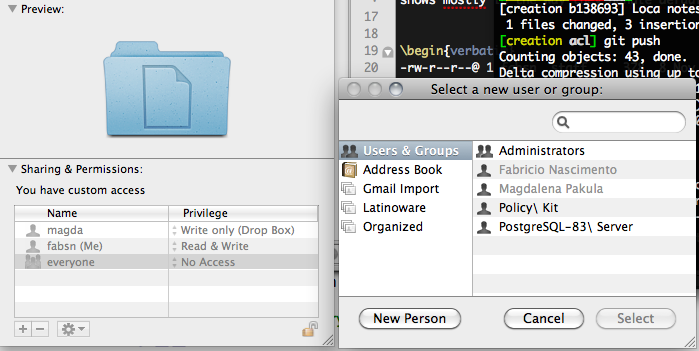
\includegraphics[height=3in]{img/mac-acl.png}
	\caption{Mac OSX Snow Leopard ACL Interface}
	\label{fig:img_mac-acl}
\end{figure}


%Parler un peut plus de Mac.


\subsection*{Using ACL in Linux}


%References 
Les dernière version des distribution Debian ou Ubuntu, comme Ubuntu 9.10, dèjá vient avec le supporte aux ACL. Dans le Ubuntu 8.10 l'application Nautilus, qui est responsable pour la visualisation du système de fichier, contenait une interface pour les ACL, apparentement l'interface a été discontinue et le Nautilus du Ubuntu 9.10 n'en y a pas encore. Les pas pour ajouter le supporte dans le Ubuntu 9.10 sont:

\begin{verbatim}
1) Installer le paquet des acl. 
user@ubuntu:$ sudo apt-get install acl
 
2) Ajouter le option 'acl' au système de fichier correcte dans le /etc/fstab, comment:
UUID='gros sequence' /dev/hda6 /home ext3 rw,auto,acl 0 1

3) Remounter le systeme de fichier avec le nouvelle option
user@ubuntu:$ sudo mount /home -o remount

\end{verbatim}

\subsection*{Ajouter ACL aux fichiers}

On peut utiliser le commande 'ls -la' pour regarde les permission. Si une fichier contient information de sécurité avancée (comme \emph{access list}) on va voir le "character" '+', comment dans le sortie du command 'ls' ci-dessous (\ref{verb:ls}). Une fichier avec '@' était dire que le fichier a quelque EAs. 

\begin{center}
\label{verb:ls}
\begin{verbatim}
-rw-r--r--@ 1 fabsn  staff     378  8 Nov 15:29 Makefile
-rw-r--r--@ 1 fabsn  staff     618  8 Nov 15:59 README
-rw-r--r--@ 1 fabsn  staff      31  8 Nov 15:15 draft-header
-rw-r--r--@ 1 fabsn  staff      24  8 Nov 15:15 header
drwxr-xr-x@ 2 fabsn  staff     102  8 Nov 15:26 img
-rw-r--r--  1 fabsn  staff     972  8 Nov 15:57 rapport-draft.aux
-rw-r--r--  1 fabsn  staff   18129  8 Nov 15:57 rapport-draft.log
drwxrwxr-x+ 3 fabsn  staff	  1024  8 Nov 20:23 repertoire
\end{verbatim}
\end{center}

Pour voir les ACL on doit utilise le commande \emph{getfacl}. Regarde que les information sont ajoute d'accord avec les définition dans l'introduction sur les ACL dans la tabelle \ref{tab:entree}. 

\begin{verbatim}
fabsn@vadmin:/media/esisar$ getfacl repertoire/
# file: repertoire/
# owner: root
# group: root
user::r-x
user:daemon:rwx
user:bin:rwx
user:fabsn:rwx
user:nobody:rwx
group::r-x
group:admin:rwx
group:fabsn:rwx
mask::rwx
other::r-x	
\end{verbatim}

Aussi on a le commande \emph{setfacl} pour modifier, ou ajouter les permission ACL. Le commande dessous par exemple modifie (-m) les permission du utilisateur \emph{fabsn} pour le répertoire. 

\begin{verbatim}
setfacl -m u:fabsn:r-x repertoire
\end{verbatim}

\subsection*{Exemple ACL d'accès}

Voici une exemple d'utilisation trouvable dans le article d'Andreas Gruembacher\cite{aclsuse}.

On parte de la création de un répertoire avec l'application de umask de valeur 027 (octal). Ça veut dire que il va   désactiver l'écriture pour le groupe propriété et l'écriture, la lecture e l'exécution pour les autres.

\begin{verbatim}
$ umask 027 
$ mkdir dir 
$ ls -dl repertoire
	drwxr-x--- ... user group ... repertoire
\end{verbatim}

La lettre "d" montre que on l'objet "répertoire" c'est une répertoire suivi pour les octet de permission "rwxr-x---". Les réticences dans le command supprime les information avec aucune pertinence pour cette exemple. Cette permission basic on toujours une représentation dans les ACL, pour les afficher on faire:

\begin{verbatim}
$ getfacl repertoire
# file: repertoire 
# owner: user 
# group: goup
user::rwx
group::r-x
other::---
\end{verbatim}

Le trois première ligne après le commande (démarrer pour le \#) nous donne les information sur les propriétaire (groupe e utilisateur) et le nom du fichier. Après chaque ligne vient la liste des ACL. Ce exemple montre une ACL minimale. Si par exemple on ajoute permissions pour le utilisateur "jean" avec le commande \emph{setfacl} on va avoir les ACL étendu.

\begin{verbatim}
$ setfacl -m user:jean:rwx repertoire
$ getfacl --omit-header repertoire 
	user::rwx 
	user:jean:rwx	
	group::r-x 
	mask::rwx 
	other::---
\end{verbatim}

Il faut rappeler que le command \emph{setfacl} a été employer avec le modificateur \emph{-m (modify)}. Pour regarder les résultat on utilisé une autre fois le \emph{getfacl}. Il faut savoir que le modificateur \emph{--omit-header} cache les première 3 ligne avec les information sur les propriétaires.  

Tout d'abord on peut voir que l'entrée masque a été ajouter avec l'entrée d'utilisateur jean. Ces permission sont crée comme la union entré les permission de jean et du groupe propriétaire. La masque doit être une valeur que ne masque aucune permission, alors, ce valeur se trouve comme l'union de les élément que définissions la classe groupe.  

\begin{verbatim}
ls -dl repertoire
	drwxrwx---+ ... user group ... repertoire
\end{verbatim}

Si on rappel le dernière exemple, le groupe propriétaire n'y a pas le droit de écriture (\emph{group::r-x}), par contre, les groupe classe vient avec ce droit. C'est pour ça que quand on calcule effectivement le droit pour le groupe propriétaire dans le modèle acl, ce droit est toujours le union avec la masque.

Le prochaine exemple montre comme lest ACL sont modifiée pour l'emploie du command \emph{chmod} ou \emph{setfacl}. On va effacer le permission de écrit de la classe groupe. On doit voir que si il n'y a pas de masque, le command doit changer directement les permission dé l'entrée ACL du groupe propriétaire. 


\begin{verbatim}
$ chmod g-w repertoire 
$ ls -dl repertoire 
	drwxr-x---+ ... user group ... repertoire 
$ getfacl --omit-header repertoire 
user::rwx 
user:jean:rwx 	#effective:r-x
group::r-x 	
mask::r-x 
other::---

\end{verbatim}

Si une ACL entrée contient permission désactivé pour le masque, getfacl doit ajouter une commentaire qui montre ça différence. Il faut voir aussi qu'est-ce que se passe quand on rajoute le permission. 

\begin{verbatim}
$ chmod g+w repertoire 
$ ls -dl repertoire 
	drwxrwx---+ ... user group ... repertoire 
$ getfacl --omit-header repertoir 
user::rwx 
user:jean:rwx 
group::r-x
mask::rwx
other::---
\end{verbatim}

Cette exemple montre que les changes avec le commande \emph{chmod} ne sont pas destructives. Les opérations sont complètement réversibles et les permission avant et après les deux opération d'aller et retour sont les mêmes, une caractéristique très important de les ACL POSIX. 

\subsection*{Exemple des ACL par défaut}

Avec le modifier -d, on peut ajouter les ACL par défaut d'un répertoire. 

\begin{verbatim}
$ setfacl -d -m group:admin:r-x repertoire 
$ getfacl --omit-header repertoire 
user::rwx
user:jean:rwx
group::r-x 
mask::rwx
other::---
default:user::rwx
default:group::r-x
default:group:admin:r-x
default:mask::r-x
default:other::---
\end{verbatim} 

Les ACL par défaut vient après les ACL d'accès et sont préfixe pour le chaîne de caractères "default::". Le courent ce que quand on ajoute une nouvelle règle seulement dans les ACL d'accès comme on a faire pour le groupe \emph{admin} aucune chose change avec les ACL par défaut. Par contre, il y a une extension sur linux que ajoute de manière automatique le règle dans les ACL par défaut. 

Il faut voir que il n y a pas aucun entrée pour jean dans les défaut ACL, alors, jean n'aura pas accès dans le nouvelle objet crée dans le répertoire (sauf si il est membre de un groupe qui a les permission). 

D'accord avec le mécanisme d'héritage qu'on a vu dans le page \ref{sec:heritage}, le sub-repertoire doit hériter les ACL de sont parent. Par défaut, le command \emph{mkdir} utilise une \emph{mode parameter} de 0777 pour ce appel de système. Observez:

\begin{verbatim}
$ mkdir repertoire/subrep 
$ getfacl --omit-header repertoire/subrep 
user::rwx 
group::r-x 
group:admin:r-x 
mask::r-x 
other::--- 
default:user::rwx 
default:group::r-x 
default:group:toolies:r-x 
default:mask::r-x 
default:other::---
\end{verbatim}

Pour les fichiers ç'arrive aussi. Le commande \emph{touch} utilise le \emph{mode value} 0666. Tous les permission que ne sont pas présent dans le \emph{mode parameter} sont écraser.

Enfin, aucune permission a été écraser dans le groupe classe, cependant, la masque a été appliqué. Ce politique s'assure que par exemple les application comme les compilateurs peuvent marcher bien avec les ACL, alors que même que ils ne supportent ce mécanisme, il peuvent créer les fichier avec les permission restreint et après les donner les permission d'exécution et quand même, les groupes et autres permission doivent marcher comme attendu. 


\section{Implèmentassions}
 
%il faut ajouter references
Les ACLs sont fréquemment implèmentèes comme extensions du noyau, c'est à dire des modules un systéme LINUX. L'objectif de cette section est d'expliquer de maniére globale l'implèmentions des ACL. 

%@@
------------------Le discussion doit lancer la base pour les èvaluations de performance et les problémes dans les sessions prochaines.----------
 
"Les ACLs sont des informations de taille variable qui sont associèes avec les objets du systéme de fichier"\cite{aclsuse}. Plusieurs implèmentations des ACLs sont possibles. Par exemple, avec Solaris, dans le systéme de fichier UFS\cite{acl_permission} chaque \emph{inode} peut avoir une ACL. S'l en a une, il doit avoir l'information \emph{i\_shadow}, un pointeur pour un \emph{shadow inode}. Les \emph{shadow inode} sont comment fichiers règuliérs d'utilisateurs. Différent fichiers avec les mÍmes ACL peut avoir pointeurs pour le mÍme \emph{shadow inodes}. Les information des ACL sont garde dans les bloc de donnèes de chaque \emph{shadow inodes}.
 
La capacitè d'associer des informations avec des fichiers est utilisè dans plusieurs fonctions du systéme de exploitation. De ce fait, la plupart des systémes \emph{UNIX-like} (de type Linux) on trouve les Attributs …tendus (\emph{Extended Attributes (EAs)}). Les ACL sont implèmentèes avec ce mècanisme.

%@@ 
La manpage \cite{aclsuse} \emph{attr(5)} contient des explications prècises sur les EAs dans Linux, ------------au notre but, suffit dire que comme les variables des processus, les EAs sont des paires (nom, valeur) associèes de maniére persistantes avec les objets du systéme de fichiers et que les appels Linux, dans le espace de utilisateur, sont employè pour opèrer sur les information de ces paires dans le espace de adresse du noyaux. Aussi pour l'implèmentation de cette infrastructure dans les systéme FreeBSD il faut voir le article de Robert Watson\cite{trust}. -------------------------------Cette article content aussi une comparaison de plusieurs implèmentation de ces systéme.
 
%@@
Dans le monde linux, ajouter le support aux ACL avec une version limitèe des EA offre plusieurs avantages: un grande facilitè d'implèmentation, ----------------opèration atomique et interface \emph{stateless} que laisse aucun surcharge à cause de les \emph{file handlers}. On verra aprés dans la section de performance, que l'efficience est assez importante pour Ítre oublier quand on parle de les donnès frèquentent accés comme les ACL.-----------------
 
\subsection{Les EAs et les systémes de fichiers}
 
Dans le monde UNIX, chaque systéme de fichier a une différent implèmentation pour les EAs. On peut penser qu'une solution partagèe pour l'ensemble des systémes pourait Ítre plus efficace. Par exemple, si on prend une solution simple où chaque objet du systéme de fichiers a les EAs, un rèpertoire avec un fichier qui a le clès EA comment le nom et le contenu comment le valeur. Cette implèmentation consommerait beaucoup de espace, ètant donnè que les blocks du systéme de fichier seront gaspillès pour conserver petit morceaux de donnè, aussi ce solution perdrait les temps pour chercher ces information a chaque accés de fichier. Aux frais de ces problémes chaque systéme tire profit de ces qualitès pour ajouter le supporte aux EAs.
 
\subsubsection*{Ext (2,3 et 4)}
 
Les ACL dans Ext suivent le principe linux: "La solution la plus simple qui marche" et pour cette raison subviennent quelques limitations. D'autres solutions existent, par contre, elle sont difficiles à ajouter au noyau de maniére satisfaisante\cite{ext_acl}.
 
La solution actuelle ajoute aux \emph{i\_node} une entrèe qui s'appelle \emph{i\_file\_acl}. Cette entrèe, si différent de 0, est une ponteur sur un bloc d'EAs. Ce bloc d'EAs a les informations de nom et valeur de tous les ACL du fichier indiquè pour cet \emph{i\_node}.
 
Le mècanisme a aussi une optimisation. Deux fichiers avec le mÍme ensemble de ACL point vers le mÍme bloc d'EAs. Le systéme garde une \emph{hash map} avec les \emph{checksum} des blocs d'EAs et leurs adresse. Chaque block a aussi un compteur de rèfèrence, comme les liens \emph{hard}. Ce mècanisme dètermine aussi que ce compteur là ne peut pas avoir plus que 1024 rèfèrences. Il s'agit d'une mesure de sècuritè en cas de perte des donnèes.
 
Aussi une limitation est imposèe: toutes les donnèes des EAs d'un fichier doivent occuper un bloc d'EAs ayant une taille de 1, 2 ou 4 KBs.
 
 
\subsubsection*{JFS}
 
Dans JFS, les EAs sont ajoutèes dans une liste consècutive de blocs contigus (un extent).  Cela veut dire que chaque paire (nom,valeur) est gardèe en sèquence et que chaque valeur de la paire ne peut pas Ítre plus grande que 64kb. Si les EAs sont assez petites, elles pourrons Ítre gardèes dans le mÍme lieu que les informations du fichier. De ce faÁon, il n'y a pas les limitations d'ext3.
 
\subsubsection*{XFS}
XFS est sans aucun dout le systéme de fichiers le plus simple pour implèmenter les EA. Les paires d'EA de petite tailles sont stockèes directement dans l'inode, celles de taille moyenne sont stockèes dans les blocs feuilles de l'arbre binaire et pour celle de grande taille, dans un arbre binaire complet.------------manque--------
XFS peut configurer la taille de sa table d'inodes. La taille minimale est de 256 octet et la taille maximale peut aller jusqu'à la moitiè des blocs du systéme de fichier. Dans le cas où on a une table de taille minimale, celle-ci n'est pas assez grande pour accueillir les ACLs. On doit alors les stocker de maniére externe ----au systéme de fichier----. Si on augmente la taille de la table les ACL pourront y Ítre stockèes. Les ACL ètant trés souvent interrogèes par le systéme, cela augmente les performances en terme de temps d'accés au dètriment de l'espace disque qu'elles consomment.
XFS n'a pas de mècanisme de partage des attributs. La taille individuelle des attributs est limitèe à 64Kb.
 
\subsubsection*{ReiserFS}

%@@

ReiserFS support le \emph{tail merging} qui permet à plusieurs fichiers de partager le mÍme bloc pour stocker leurs donnèes. Cela rend le systéme trés efficace pour s'il on posséde de nombreux fichiers de petite taille. De l'autre cÙtè cette technique consomme beaucoup de ressources CPU. 

Comme le ReiserFs peut facilement manipuler des petits fichiers, les EA peuvent Ítre implèmentèes sous forme de petits fichiers. Pour chaque fichiers qui a un EA, un dossier spècial (qui est souvent cachè) est crèè avec un nom dèrivè de son inode. Dans ce dossier chaque EA est stockèe dans un fichier sèparè qui a pour nom le nom de l'attribut. Le contenu de chaque fichier est la valeur de l'attribut.

Le systéme ReiserFS n'implèmente pas le partage d'attributs mais la crèation d'une extension pour le gèrer est possible. La taille individuelle des attributs est limitèe à 64Kb.

%@@
----------------------Sharing could even be implemented
on a per-attribute bases, so the result would be
a highly efficient and flexible solution. --------------The size of individual
attributes is limited to 64 KiB.

\subsubsection*{HGFS+}

%@@
\section*{Système de Fichier Remote}
%@@
\subsubsection*{Samba}
%@@

\subsubsection*{NFS}
%@@
\section*{Problèmes}

\subsection*{Compatibilité}

Il y deux situation qui devons être considère quand on parle de j'ajutage les nouvelle fonctionnalité aux système de fichiers et consequentent au noyaux: les mises a jour et comme le système qui ne sont pas mise a jour répondre.
Aussi il faut qu'on sache que quand on a besoin de un noyaux plus léger, par exemple pour démarré le système de récupération, et que dans cette cas on ne veut pas avoir les EAs dans le noyaux. 

Tous les système de fichier que n'avons pas le supporte a les ACl activé on a mécanisme de mis en place le supporte dans le moment de montage or automatiquement dans le première use de les EAs, sans l'interférence d'utilisateur. 

On espère que les vieux version du noyaux n'arrêtions pas de marcher avec les ACL. Dans un noyaux on les ACL ne sont pas supporté, les système de fichiers que implementent les ACL dans les répertoire , comme le ReiserFS, devient venir visible. Il faut quand même que les droit de permission de ces fichiers sont configure de façon que les utilisateurs ne peuvent pas changer les information de manière inadéquat. Un autre exemple c'est avec le système de fichier ext2 et ext3, si on effacer les fichier avec les ACL dans le kernel sans les support les information des ACL ne seront pas effacer, alors, on peut exécuter manuellement la vérification du système après pour mettre a jour les information. 
 	
Aussi le mécanisme de héritage ne marcherai pas. 

\subsection*{Copie de Sécurité}

Un aspect très important et usuellement oublier sont les copie de sécurité. Les outils comment \emph{cpio} et \emph{tar} ne connait pas les ACL. Ça veut dire que quand on doit garder notre information, si on en faire avec ces outils on perdra les EAs.

Une format appelle \emph{pax (Portable Archive Interchange)} a été défini pour POSIX pour résoudre ce problème. Le outil \emph{pax} peut comprendre les format de \emph{cpio} et \emph{tar} et aussi le nouveaux format \emph{pax}. Ce nouveau format a les \emph{extended headers} que peuvent décrire les EAs. Le outil \emph{tar} peut le lire par contre il doit perdre les information de ACL. 

On peau aussi utiliser \emph{getfacl} et \emph{setfacl} comment outils pour faire les copie de les droits d'accès, par contre, c'est pas pratique de les user si on a pas une copie de sécurité complète, mais quelques fichiers. \section*{Conclusion}

\newpage

% Le utilisateurs
% le complication atacher
\begin{thebibliography}{9}
 
\bibitem{aclsuse}
  Andreas Gruenbacher,
  \emph{POSIX Acess Control Lists on Linux}.
  http://www.suse.de/~agruen/acl/linux-acls/online/,
  2003.

\bibitem{ieee1}
    IEEE Std 1003.1-2001 (Open Group Technical Standard, Issue 6), 
	Standard for Information Technology--Portable Operating System Interface (POSIX) 2001. 
	ISBN 0-7381-3010-9. 
	http://www.ieee.org/

\bibitem{ieee2}
    IEEE 1003.1e and 1003.2c: Draft Standard for Information Technology--Portable Operating System Interface (POSIX)--Part 1: System Application Program Interface (API) and Part 2: Shell and Utilities, draft 17 (withdrawn). 
	October 1997. 
	http://wt.xpilot.org/publications/posix.1e/

\bibitem{ftp}
	Mark Lowes: 
	Proftpd: 
	A User's Guide March 31, 2003. 
	http://proftpd.linux.co.uk/

\bibitem{posix17}
    Winfried Trümper: Summary about Posix.1e. Publicly available copies of POSIX 1003.1e/1003.2c. February 28, 1999. http://wt.xpilot.org/publications/posix.1e/

\bibitem{acl_permission}
	Jim Mauro: Controlling permissions with ACLs. Describes internals of UFS's shadow inode concept. SunWorld Online, June 1998.

\bibitem{trust}
	Robert N. M. Watson: Introducing Supporting Infrastructure for Trusted Operating System Support in FreeBSD. BSDCon 2000, Monterey, CA, September 8, 2000. http://www.trustedbsd.org/docs.html
	
\bibitem{nfs_problem}
	Andreas Grünbacher: Linux Extended Attributes and ACLs. Session "Known Problems and Bugs". http://acl.bestbits.at/problems.html
	
\bibitem{ext_acl}
	Andreas Dilger: [RFC] new design for EA on- disk format. Mailing list communication, July 10, 2002. http://acl.bestbits.at/pipermail/acl-devel/ 2002-July/001077.html
	
\bibitem{ext_jfs}
	Austin Common Standards Revision Group. http: //www.opengroup.org/austin/

\end{thebibliography}

\end{document}
